\section{Chemical equations and formulas}
\subsection{Chemical equations}

\subsection{Using Chemfig package}
\begin{frame}
	The \lp{chemfig} provides commands to draw compound structures, e.g.

	\codex{Simple $H_2O$}{chemfig-h2o}
\end{frame}
\begin{frame}
	\codex{Specify bond with \lcs{chemfig}}{chemfig-bonds}
\end{frame}
\begin{frame}
	\codex{The chemfig-angle system}{chemfig-angles}
	\codex{Water rotated by 90\celsius{}}{chemfig-h2o-spinned}
\end{frame}
\begin{frame}
	\codex{Drawing more complex structures}{chemfig-keep-start}
\end{frame}
\begin{frame}
	\codex{Circle construction}{chemfig-circle}

	Using the \lcs{lewis} the eletrons are noted:
	\code{ \lcs{lewis}\{<angle\_index><state>,<atom>\}}
\end{frame}
\subsection{Naming of compounds}
\begin{frame}
	\codex{Display names under compounds}{chemfig-chemname}
	\code{ \lcs{chemname}\{ structure using \lcs{chemfig} \}\{name\} }
\end{frame}

\subsection{Writing chemical formulas}
\begin{frame}
	\codex{Chemical equations}{chemfig-eqn}
	\lcs{chemsign} renders signs while \lcs{chemrel} the relation
	\begin{mitemize}
		\item $->$ \chemrel{->}
		\item $<-$ \chemrel{<-}
		\item $<->$ \chemrel{<->}
	\end{mitemize}
\end{frame}

\begin{frame}
	\codex{More complex arrows with full scheme support}{chemfig-eqn-scheme}

	More options for \lcs{arrow}
	\begin{mitemize}
		\item $=>$ \item $<=$ \item $<=>>$
	\end{mitemize}
	for more see \href{http://www.ctan.org/pkg/chemfig}{Chemfig-Documentation page
	53}
\end{frame}

\begin{frame}
	\codex{Arrow with additional arguments}{chemfig-eqn-arrow}
	Note that names can also be placed in this environment.
\end{frame}


\subsection{Graphical editing}
\begin{frame}
	\begin{center}
		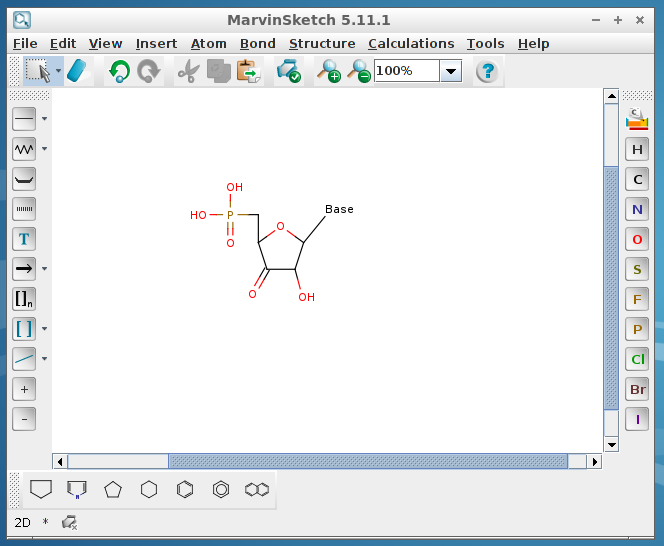
\includegraphics[width=0.5\textwidth]{ss-marvin-sketch.png}
		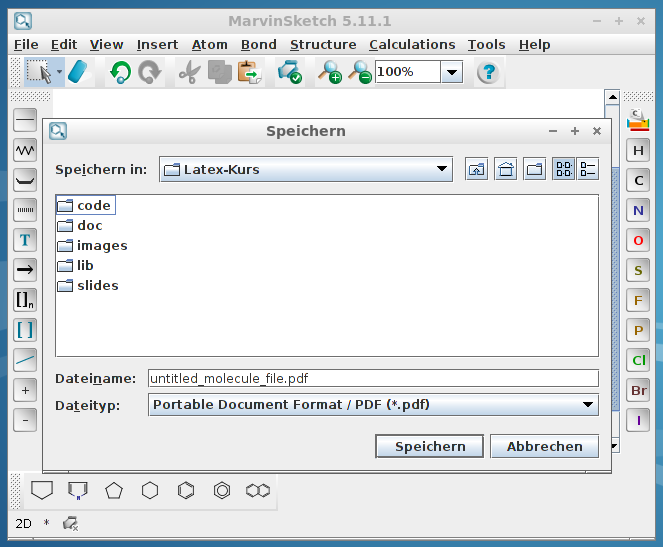
\includegraphics[width=0.5\textwidth]{ss-marvin-sketch-2.png}
	\end{center}
	ChemAxons Marvin Suite\footnote{\url{http://www.chemaxon.com}} (including Sketch) is freely available for academic
	use (Java).
\end{frame}

